\documentclass[12pt, a4paper]{article}

% ─── Pacotes essenciais ───────────────────────────────────────────────────────
\usepackage[utf8]{inputenc}
\usepackage[T1]{fontenc}
\usepackage[brazil]{babel}
\usepackage{lmodern}

% Layout
\usepackage[top=3cm, bottom=2cm, left=3cm, right=2cm]{geometry}
\usepackage{setspace}
\onehalfspacing

% Matemática
\usepackage{amsmath, amssymb, amsthm}

% Figuras e tabelas
\usepackage{graphicx}
\usepackage{float}
\usepackage{booktabs}
\usepackage{caption}
\usepackage{subcaption}
\usepackage{longtable}

% Algoritmos / código
\usepackage{algorithm}
\usepackage{algpseudocode}
\usepackage{listings}
\usepackage{xcolor}

% Referências e links
\usepackage[colorlinks=true, linkcolor=blue, citecolor=blue, urlcolor=blue]{hyperref}
\usepackage[backend=biber, style=abnt]{biblatex}
\addbibresource{referencias.bib}

% Outros
\usepackage{enumitem}
\usepackage{multirow}
\usepackage{array}
\usepackage{pdflscape}
\usepackage{lipsum}   % remover no documento final

% ─── Configuração de listings ─────────────────────────────────────────────────
\lstset{
  basicstyle=\ttfamily\small,
  keywordstyle=\color{blue}\bfseries,
  commentstyle=\color{gray},
  stringstyle=\color{orange},
  numbers=left,
  numberstyle=\tiny,
  frame=single,
  breaklines=true,
  captionpos=b,
}

% ─── Dados do projeto ─────────────────────────────────────────────────────────
\newcommand{\disciplina}{PRO3341 -- Modelagem e Otimização de Sistemas de Produção}
\newcommand{\professora}{Prof\textsuperscript{a}. Dra. Celma O. Ribeiro}
\newcommand{\semestre}{1\textsuperscript{o} Semestre de 2026}
\newcommand{\tituloProj}{[Título do Projeto]}   % ← preencher
\newcommand{\empresa}{[Nome da Empresa]}         % ← preencher
\newcommand{\grupoA}{Aluno 1}                    % ← preencher
\newcommand{\grupoB}{Aluno 2}
\newcommand{\grupoC}{Aluno 3}
\newcommand{\grupoD}{Aluno 4}                    % remover se grupo de 3

% ─── Documento ────────────────────────────────────────────────────────────────
\begin{document}

% Capa
% ─── Capa ────────────────────────────────────────────────────────────────────
\begin{titlepage}
  \centering

  \vspace*{1cm}
  {\large \textbf{Universidade de São Paulo}}\\
  {\large Escola Politécnica}\\
  {\large Departamento de Engenharia de Produção}\\[1.5cm]

  {\large \disciplina}\\[0.3cm]
  {\large \professora}\\[0.3cm]
  {\large \semestre}\\[2.5cm]

  {\LARGE \textbf{\tituloProj}}\\[1cm]

  {\large Empresa parceira: \textbf{\empresa}}\\[3cm]

  \begin{flushleft}
    {\large \textbf{Grupo:}}\\[0.3cm]
    {\large \grupoA}\\
    {\large \grupoB}\\
    {\large \grupoC}\\
    {\large \grupoD}\\   % remover se grupo de 3
  \end{flushleft}

  \vfill
  {\large São Paulo, \today}
\end{titlepage}
\newpage


% Sumário
\tableofcontents
\newpage

% Relatórios — descomente conforme entrega
%==============================================================================
%  RELATÓRIO 1  —  Entregue em 24/03/2026
%==============================================================================

\section{Relatório 1: Caracterização da Empresa e do Problema}

\subsection{Sobre a Empresa}

A Rentex é uma empresa do setor têxtil fundada em 1991, com sede na Rua João
Antônio de Oliveira, 1083, no bairro de Mooca/Belenzinho, São Paulo
(CEP 03111-001). Com cerca de 30 funcionários distribuídos em dois turnos, opera
no segmento B2B fabricando tecidos planos para confecção e uniformes. O contato
institucional para este projeto é Pedro Charmillot Silva, Diretor de Novos
Negócios, cuja autorização de uso da empresa para fins acadêmicos encontra-se
no Anexo~A.

A empresa é especializada em sarjas e forros, atendendo fabricantes de vestuário
que demandam materiais com composições específicas de algodão, poliéster e
elastano. Seu modelo comercial é baseado em parcerias de longo prazo: parte da
produção é comprometida semanalmente com clientes fixos por contrato.

\subsubsection{Portfólio de Produtos}

O portfólio ativo compreende quatro famílias:

\textbf{Sarja Barcelos (100\% algodão)} é o produto de maior volume da linha,
com processo mais padronizado e tempo de setup reduzido nos teares. Atende
principalmente confecção básica e uniformes. Sua margem unitária é a menor entre
as sarjas.

\textbf{Sarja Joy (mista poliéster/elastano)} tem composição aproximada de
70\% algodão, 25\% poliéster e 5\% elastano, o que exige troca de urdume e
trama nos teares a cada novo lote. O tempo de setup é significativamente maior,
mas a margem de contribuição compensa.

\textbf{Forro de Poliéster Padrão (100\% poliéster)} é um forro leve de
acabamento padronizado usado no interior de roupas e bolsas. Processo rápido,
alto volume, menor margem. Três clientes têm contrato de fornecimento mínimo
semanal para este produto.

\textbf{Forro de Poliéster Premium (95\% poliéster/5\% elastano)} é a variação
de maior valor do forro padrão, com acabamento acetinado voltado ao segmento de
moda feminina. Um cliente estratégico tem contrato de mínimo semanal.

\subsection{Definição do Problema}

Com cinco teares planos e armazenamento limitado de matéria-prima, a Rentex não
consegue atender simultaneamente toda a demanda de mercado de todos os produtos.
Toda semana o gerente de produção decide quanto produzir de cada tecido, e essa
decisão tem impacto direto no resultado financeiro.

O conflito central está entre os forros e as sarjas. Os forros têm alta demanda
e processo rápido, mas margem baixa, e parte da produção é obrigatória por
contrato. As sarjas têm setup mais demorado e menor demanda, mas margem
substancialmente maior. Produzir mais forro do que o necessário consome horas de
tear que poderiam gerar receita maior nas sarjas; produzir exclusivamente sarjas
significaria quebrar contratos com clientes de longo prazo.

O problema é, portanto, determinar o mix semanal que maximize a margem de
contribuição total sujeita às restrições de capacidade dos teares, de estoque
de matéria-prima, de mão de obra e de demanda.

\subsection{Concepção da Modelagem}

O problema se enquadra naturalmente em um modelo de Programação Linear. A
variável de decisão $x_j$ representa a quantidade de lotes de 100 metros do
produto $j$ a produzir por semana. A função objetivo maximiza a soma das margens
de contribuição, calculadas como preço de venda menos custos variáveis diretos
de cada produto.

Os parâmetros do modelo incluem os tempos de ciclo dos teares (com setup
amortizado sobre o tamanho mínimo de lote contratual), os coeficientes de
consumo de cada matéria-prima por lote e a disponibilidade semanal de cada
recurso, calculada a partir dos dois turnos de trabalho menos paradas programadas.

As restrições são de cinco tipos. A capacidade dos teares limita o total de
horas de máquina utilizadas por semana. Os estoques de algodão, poliéster e
elastano impõem limites ao consumo de cada insumo. A mão de obra disponível
dos 30 funcionários restringe as horas-homem semanais, mesmo com margem para
horas extras dentro dos limites da convenção coletiva. Os contratos de
fornecimento impõem quantidades mínimas semanais para os dois forros. Por fim,
os limites de demanda máxima de mercado definem o teto de produção para cada
família.

\subsection{Viabilidade do Projeto}

Os dados necessários para a formulação estão disponíveis no sistema de gestão
da empresa: roteiros de fabricação, relatórios de capacidade, fichas de custo e
histórico de pedidos. A Rentex confirmou, por intermédio de Pedro Charmillot
Silva, a disponibilidade de acesso a essas informações durante o desenvolvimento
do projeto. A formulação matemática completa e os primeiros resultados
computacionais serão apresentados no Relatório~2.

\subsection{Artigo de Referência}

O artigo selecionado é:

\begin{quote}
SOBREIRO, V. A.; NAGANO, M. S. Proposta de uma heurística construtiva baseada
na TOC para definição de mix de produção. \textit{Produção}, v.~23, n.~3,
p.~468--477, jul./set. 2013.
\end{quote}

O artigo aborda o mesmo problema estrutural da Rentex: múltiplos produtos
competindo por recursos produtivos insuficientes para atender toda a demanda,
com objetivo de maximizar o ganho total. Os autores utilizam a solução ótima
da Programação Linear Inteira como referência de qualidade e propõem heurísticas
construtivas baseadas na Teoria das Restrições para instâncias de maior escala.
A conexão com a metodologia adotada neste projeto é discutida em detalhe no
Relatório~2. O artigo completo encontra-se no Anexo~B.

\newpage

\subsection*{Anexo A -- Autorização da Empresa}

\begin{figure}[H]
\centering

\includegraphics[width=0.80\textwidth]{relatorio1/carta_empresa.pdf}
\caption{Autorização emitida pela Rentex Indústria Têxtil LTDA, contendo nome,
         cargo e telefone de contato do responsável, Pedro Charmillot Silva,
         Diretor de Novos Negócios (+55~11~99858-1812).}
\end{figure}

\newpage

\subsection*{Anexo B -- Artigo de Referência}

\foreach \pg in {1,2,3,4,5,6,7,8,9,10}{%
  \includegraphics[width=\textwidth, page=\pg]{relatorio1/artigo_referencia.pdf}%
  \newpage
}

%%==============================================================================
%  RELATÓRIO 2  —  Entrega: 13/05/2026
%==============================================================================

\section{Relatório 2: Formulação Matemática e Primeiros Resultados}

\subsection{Introdução}

Este relatório apresenta a segunda etapa do projeto. Com base na concepção
do Relatório 1, são apresentados: a revisão bibliográfica que fundamenta a
técnica, a formulação matemática completa e aprimorada do modelo de
Programação Linear para o problema de mix de produção da Rentex, e os
primeiros resultados computacionais com análise preliminar.

A formulação foi enriquecida em relação à concepção inicial para capturar o
elemento central do problema: o \textbf{trade-off entre maximizar margem de
contribuição no curto prazo e manter parcerias de longo prazo com clientes
contratuais de menor margem}. Esse elemento distingue o problema da Rentex de
um simples problema de alocação, tornando o uso de Programação Linear
genuinamente necessário para derivar a política ótima.

\newpage

\subsection{Conexão com o Artigo de Referência}

O artigo de \textcite{sobreiro2013}, ``Proposta de uma heurística construtiva
baseada na TOC para definição de mix de produção'', publicado na revista
\textit{Produção} (Qualis A2), é diretamente aplicável ao problema da Rentex.
Esta seção explicita as conexões e o que da metodologia do artigo será utilizado.

\subsubsection{Paralelo entre o Artigo e o Problema Rentex}

O problema tratado por \textcite{sobreiro2013} é, na sua forma geral:

\begin{align}
  &\text{Maximizar} \quad Z = \sum_{j=1}^{n} (P_j - c_j)\, x_j \nonumber \\
  &\text{s.a.} \quad \sum_{j=1}^{n} a_{ij}\, x_j \leq b_i, \quad i = 1, \ldots, m \nonumber \\
  &\phantom{\text{s.a.}} \quad x_j \leq d_j, \quad j = 1, \ldots, n \nonumber
\end{align}

A estrutura é idêntica ao caso Rentex: maximizar a soma das margens de contribuição
sujeita a restrições de capacidade dos recursos e limites de demanda. O problema
da Rentex adiciona restrições de demanda mínima contratual e variáveis de
penalidade por subatendimento, conforme detalhado na seção de formulação.

\subsubsection{O que o Artigo Usa e o que Este Trabalho Adota}

\textcite{sobreiro2013} propõem uma \textbf{heurística construtiva} baseada em
dois elementos: (i) a Teoria das Restrições (TOC), para identificar o recurso
gargalo e ordenar produtos por eficiência no gargalo; e (ii) o problema da
mochila (\textit{knapsack}), para alocar a capacidade disponível de forma gulosa.
O artigo compara sua heurística com a \textbf{solução ótima da Programação Linear
Inteira (PLI)}, que é adotada como referência (\textit{benchmark}).

Este projeto adota uma abordagem diferente e complementar:

\begin{enumerate}[label=\textbf{(\roman*)}]
  \item \textbf{Identificação do gargalo via TOC} (do artigo): a análise da
        eficiência por hora de tear de cada produto -- análoga ao índice
        $R_i = \mathrm{CM}_i / t_{i,\mathrm{BN}_k}$ do artigo -- é usada para
        interpretar a solução ótima e explicar por que certos produtos são
        priorizados.

  \item \textbf{PL como solução exata} (em vez da heurística): como o problema
        tem apenas 4 produtos e 5 recursos, a PL encontra o ótimo global em
        fração de segundo, tornando desnecessária a heurística do artigo. A PL
        é exatamente o \textit{benchmark} que o artigo usa para validar suas
        heurísticas -- estamos operando no patamar de referência máxima.

  \item \textbf{Extensão do modelo com penalidade de relacionamento}: o artigo
        não modela o valor de parcerias de longo prazo. Este projeto incorpora
        variáveis de shortfall e penalidades na função objetivo, o que torna o
        problema não trivial e responde à pergunta gerencial central: \textit{quanto
        vale produzir produtos menos rentáveis para manter parcerias de longo prazo?}

  \item \textbf{Análise de sensibilidade paramétrica}: o artigo sugere como
        trabalho futuro a aplicação das heurísticas em situações práticas e a
        análise de sensibilidade. Este trabalho realiza exatamente isso,
        quantificando o threshold de penalidade a partir do qual o modelo
        recomenda honrar o nível preferido dos clientes contratuais.
\end{enumerate}

\newpage

\subsection{Revisão Bibliográfica}

\subsubsection{O Problema de Mix de Produção com Restrições de Relacionamento}

O problema de definição do mix de produção consiste em determinar as quantidades
a fabricar de cada produto em um horizonte fixo, maximizando a margem de
contribuição total, respeitando as capacidades dos recursos e os limites de
demanda \cite{hillier2006, arenales2007}. Quando existe demanda mínima contratual
e penalidade por subatendimento, o problema passa a capturar o valor das
relações comerciais de longo prazo, tornando-o mais rico e gerencialmente relevante.

\textcite{sobreiro2013} demonstram que, para instâncias de pequeno porte (até
8 produtos e 4 gargalos), a Programação Linear Inteira encontra a solução ótima
em menos de 1 segundo, o que confirma a adequação da PL para o problema da Rentex.

\subsubsection{Programação Linear como Técnica Principal}

A Programação Linear é selecionada por três razões:

\begin{enumerate}[label=\textbf{(\alph*)}]
  \item \textbf{Optimalidade garantida:} o método Simplex encontra o ótimo global
        para qualquer problema LP, ao contrário de heurísticas \cite{hillier2006}.

  \item \textbf{Análise de sensibilidade nativa:} preços-sombra e intervalos de
        ranging emergem diretamente da solução ótima, fornecendo informação
        gerencial sobre o valor marginal de capacidade adicional e sobre a
        robustez do plano a variações nos parâmetros \cite{winston2002}.

  \item \textbf{Escalabilidade para o modelo aprimorado:} a extensão com
        variáveis de shortfall e penalidades mantém a estrutura LP, sem necessitar
        de PLIM, graças à linearidade da penalidade.
\end{enumerate}

\subsubsection{Teoria das Restrições e Gargalo}

A TOC \cite{goldratt2006} identifica que o desempenho do sistema é determinado
por seu gargalo. No contexto da PL, o gargalo é o recurso com maior preço-sombra.
\textcite{sobreiro2013} formalizam a eficiência de cada produto em relação ao
gargalo como $e_j = \mathrm{MC}_j / a_{\text{garg},j}$, que é exatamente o
critério usado neste trabalho para interpretar a priorização dos produtos.

\subsubsection{Modelagem do Valor de Parcerias de Longo Prazo}

A literatura de gestão de operações reconhece que em mercados B2B a relação com
clientes de longo prazo tem valor que vai além da margem de contribuição imediata.
\textcite{arenales2007} discutem como restrições de compromisso mínimo devem
ser incorporadas a modelos de PL para planejamento da produção em empresas com
contratos de fornecimento estável. A abordagem de penalidade por shortfall
adotada neste trabalho transforma as restrições de mínimo contratual de
\textit{hard constraints} em soft constraints parametrizadas, permitindo que o
modelo responda à pergunta: a que custo de margem de contribuição imediata
vale honrar o nível preferido pelo cliente?

\newpage

\subsection{Coleta e Validação dos Dados}

Os dados foram coletados em levantamento conduzido junto ao PCP da Rentex em
abril de 2026, a partir de: roteiros de fabricação do sistema de gestão, relatórios
de capacidade dos últimos doze meses, fichas de custo de produto e histórico de
pedidos dos últimos seis meses.

\subsubsection{Capacidades Semanais Disponíveis}

\begin{table}[H]
\centering
\caption{Capacidades semanais disponíveis validadas}
\label{tab:cap_r2}
\begin{tabular}{clrrc}
\toprule
\textbf{$i$} & \textbf{Recurso} & \textbf{Bruto} & \textbf{Eficiência} & \textbf{$b_i$} \\
\midrule
1 & Teares (h/semana)              & 448 h   & 84,8\% & \textbf{380 h}   \\
2 & Fio de algodão (kg/semana)     & 400 kg  & 100\%  & \textbf{400 kg}  \\
3 & Fio de poliéster (kg/semana)   & 500 kg  & 100\%  & \textbf{500 kg}  \\
4 & Elastano (kg/semana)           &  12 kg  & 100\%  & \textbf{12 kg}   \\
5 & Mão de obra direta (h/semana)  & 1.440 h & 83,3\% & \textbf{1.200 h} \\
\bottomrule
\multicolumn{5}{l}{\footnotesize Bruto dos teares = 5 teares $\times$ 2 turnos $\times$ 8 h $\times$ 5,6 dias úteis médios.}
\end{tabular}
\end{table}

\subsubsection{Produtos, Margens e Níveis de Demanda}

\begin{table}[H]
\centering
\caption{Margens de contribuição e níveis de demanda semanal}
\label{tab:prod_r2}
\begin{tabular}{llrrrrrr}
\toprule
\textbf{$j$} & \textbf{Produto} & \textbf{Preço} & \textbf{CV} & \textbf{MC$_j$} & \textbf{$d^{\min}$} & \textbf{$d^{\text{pref}}$} & \textbf{$d^{\max}$} \\
\midrule
1 & Sarja Barcelos  & 1.800 & 1.100 & \textbf{700}  &   0 & ---  & 200 \\
2 & Sarja Joy       & 2.400 & 1.400 & \textbf{1.000}&   0 & ---  &  80 \\
3 & Forro Padrão    &   600 &   380 & \textbf{220}  &  60 & \textbf{130} & 160 \\
4 & Forro Premium   &   900 &   550 & \textbf{350}  &  20 & \textbf{45}  &  60 \\
\bottomrule
\multicolumn{8}{l}{\footnotesize $d^{\min}$: contrato mínimo inegociável. $d^{\text{pref}}$: nível esperado pelo cliente contratual.}\\
\multicolumn{8}{l}{\footnotesize CV e MC em R\$/lote de 100~m lineares.}
\end{tabular}
\end{table}

\subsubsection{Coeficientes Técnicos}

\begin{table}[H]
\centering
\caption{Coeficientes técnicos $a_{ij}$ (consumo de recurso por lote)}
\label{tab:coef_r2}
\renewcommand{\arraystretch}{1.2}
\begin{tabular}{lcccc}
\toprule
\textbf{Recurso $i$} & \textbf{S. Barcelos} & \textbf{S. Joy} & \textbf{F. Padrão} & \textbf{F. Premium} \\
\midrule
Teares (h/lote) incl. setup & 0,85 & 1,40 & 0,50 & 0,70 \\
Fio algodão (kg/lote)       & 1,35 & 0,95 & 0,00 & 0,00 \\
Fio poliéster (kg/lote)     & 0,00 & 0,35 & 1,60 & 1,55 \\
Elastano (kg/lote)          & 0,00 & 0,07 & 0,00 & 0,08 \\
MOD (h/lote)                & 0,40 & 0,65 & 0,25 & 0,35 \\
\bottomrule
\end{tabular}
\end{table}

O coeficiente de teares incorpora o tempo de setup amortizado pelo tamanho mínimo
de lote contratual (50~m para a Barcelos, 80~m para a Joy), conforme descrito
no Relatório 1.

\newpage

\subsection{Formulação Matemática Final}
\label{sec:form_final}

\subsubsection{Por que o Modelo Básico é Insuficiente}

Um modelo com apenas demanda mínima contratual como \textit{hard constraint}
($x_j \geq d_j^{\min}$) produz um resultado trivialmente previsível: o Simplex
alocaria toda a capacidade de tear aos produtos de maior eficiência (sarjas) e
produziria exatamente o mínimo contratual dos forros. Essa solução dispensa o uso
de um modelo de otimização, pois pode ser obtida por inspeção direta da tabela de
eficiências.

O elemento que torna o problema não trivial é a existência de um \textbf{nível
preferido} pelo cliente -- abaixo do qual existe risco de perda da parceria --
que está acima do mínimo contratual legal. A Rentex precisa decidir: quanto de
margem de contribuição imediata vale sacrificar para honrar o nível preferido e
preservar a relação de longo prazo? Essa é uma decisão de trade-off contínuo
que a Programação Linear é capaz de formalizar e resolver.

\subsubsection{Variáveis de Decisão}

\begin{description}[leftmargin=3cm]
  \item[$x_j \geq 0$] quantidade de lotes do produto $j$ a produzir por semana.
  \item[$s_j^- \geq 0$] \textit{shortfall}: lotes entregues abaixo do nível preferido
        pelo cliente do produto $j$ (definido somente para os produtos com contrato,
        $j \in \{3, 4\}$).
\end{description}

\subsubsection{Parâmetros Adicionais}

\begin{description}[leftmargin=3cm]
  \item[$d_j^{\text{pref}}$] nível de produção preferido pelo cliente contratual
        do produto $j$. Abaixo desse nível, o cliente percebe subatendimento.
  \item[$\rho_j$] penalidade por lote de shortfall (R\$/lote): custo esperado de
        relacionamento por cada lote produzido abaixo de $d_j^{\text{pref}}$.
        Representa o valor semanal amortizado do risco de perda da parceria.
\end{description}

A penalidade $\rho_j$ é calculada como:
\begin{equation}
  \rho_j = \frac{V_j \cdot \pi_j}{52 \cdot \overline{s}_j}
  \label{eq:rho}
\end{equation}
onde $V_j$ é o valor anual do contrato, $\pi_j$ é a probabilidade estimada de
perda do cliente por semana de subatendimento, e $\overline{s}_j$ é o shortfall
esperado por semana de subatendimento. O parâmetro $\rho_j$ é tratado como
variável nos cenários de análise de sensibilidade.

\subsubsection{Modelo de Programação Linear Aprimorado}

\textbf{Função objetivo:}
\begin{equation}
  \max \quad Z = \underbrace{\sum_{j=1}^{4} \mathrm{MC}_j \, x_j}_{\text{MC total bruta}}
                - \underbrace{\sum_{j \in \{3,4\}} \rho_j \, s_j^-}_{\text{custo de relacionamento}}
  \label{eq:fo_r2}
\end{equation}

\textbf{Restrições de capacidade:}
\begin{align}
  0{,}85\,x_1 + 1{,}40\,x_2 + 0{,}50\,x_3 + 0{,}70\,x_4 &\leq 380
    \tag{R1 -- Teares} \label{eq:tear}\\
  1{,}35\,x_1 + 0{,}95\,x_2 &\leq 400
    \tag{R2 -- Fio algodão} \\
  0{,}35\,x_2 + 1{,}60\,x_3 + 1{,}55\,x_4 &\leq 500
    \tag{R3 -- Fio poliéster} \\
  0{,}07\,x_2 + 0{,}08\,x_4 &\leq 12
    \tag{R4 -- Elastano} \\
  0{,}40\,x_1 + 0{,}65\,x_2 + 0{,}25\,x_3 + 0{,}35\,x_4 &\leq 1200
    \tag{R5 -- MOD}
\end{align}

\textbf{Restrições de relacionamento (soft constraints):}
\begin{equation}
  x_j + s_j^- \geq d_j^{\text{pref}}, \quad j \in \{3, 4\}
  \label{eq:soft}
\end{equation}

\textbf{Restrições de demanda:}
\begin{equation}
  x_j \geq d_j^{\min}, \quad x_j \leq d_j^{\max}, \quad \forall j
  \label{eq:dem}
\end{equation}

\textbf{Não negatividade:}
\begin{equation}
  x_j \geq 0, \quad s_j^- \geq 0, \quad \forall j
\end{equation}

O modelo tem \textbf{6 variáveis de decisão} (4 de produção + 2 de shortfall),
\textbf{5 restrições de capacidade}, \textbf{2 soft constraints} de relacionamento
e \textbf{8 restrições de demanda}, totalizando 15 restrições funcionais.

\subsubsection{Verificação de Não Trivialidade}

O plano que atende toda a demanda máxima viola a restrição de teares:
\[
  0{,}85(200) + 1{,}40(80) + 0{,}50(160) + 0{,}70(60)
  = 170 + 112 + 80 + 42 = \mathbf{404 \; \text{h}} > 380 \; \text{h} \quad \times
\]
O modelo não tem solução trivial. Além disso, o nível preferido dos forros
($d_3^{\text{pref}} = 130$, $d_4^{\text{pref}} = 45$) gera um trade-off real:
honrar esses níveis requer realocar horas de tear que de outra forma seriam usadas
para aumentar a produção dos forros ou das sarjas, conforme detalhado na análise.

\newpage

\subsection{Implementação Computacional}
\label{sec:impl}

\begin{lstlisting}[caption={Modelo PL aprimorado da Rentex -- \texttt{rentex\_pl.py}},
                   label={lst:rentex}]
"""
PRO3341 - Projeto Rentex: Mix de Producao com Trade-off de Parcerias
"""
import pulp

produtos   = ['Sarja_Barcelos','Sarja_Joy','Forro_Padrao','Forro_Premium']
recursos   = ['Teares','Fio_Algodao','Fio_Poliester','Elastano','MOD']
contratos  = ['Forro_Padrao','Forro_Premium']

MC     = {'Sarja_Barcelos':700,'Sarja_Joy':1000,'Forro_Padrao':220,'Forro_Premium':350}
b      = {'Teares':380,'Fio_Algodao':400,'Fio_Poliester':500,'Elastano':12,'MOD':1200}
a      = {
    'Teares':       {'Sarja_Barcelos':0.85,'Sarja_Joy':1.40,
                     'Forro_Padrao':0.50,'Forro_Premium':0.70},
    'Fio_Algodao':  {'Sarja_Barcelos':1.35,'Sarja_Joy':0.95,
                     'Forro_Padrao':0.00,'Forro_Premium':0.00},
    'Fio_Poliester':{'Sarja_Barcelos':0.00,'Sarja_Joy':0.35,
                     'Forro_Padrao':1.60,'Forro_Premium':1.55},
    'Elastano':     {'Sarja_Barcelos':0.00,'Sarja_Joy':0.07,
                     'Forro_Padrao':0.00,'Forro_Premium':0.08},
    'MOD':          {'Sarja_Barcelos':0.40,'Sarja_Joy':0.65,
                     'Forro_Padrao':0.25,'Forro_Premium':0.35},
}
d_min  = {'Sarja_Barcelos':0,'Sarja_Joy':0,'Forro_Padrao':60,'Forro_Premium':20}
d_max  = {'Sarja_Barcelos':200,'Sarja_Joy':80,'Forro_Padrao':160,'Forro_Premium':60}
d_pref = {'Forro_Padrao':130,'Forro_Premium':45}

def resolver(rho, b_ov=None):
    _b = {**b, **(b_ov or {})}
    prob = pulp.LpProblem("Rentex", pulp.LpMaximize)
    x = {j: pulp.LpVariable(f"x_{j}", lowBound=0) for j in produtos}
    s = {j: pulp.LpVariable(f"s_{j}", lowBound=0) for j in contratos}

    # Funcao objetivo: MC bruta menos custo de relacionamento
    prob += (pulp.lpSum(MC[j]*x[j] for j in produtos)
             - pulp.lpSum(rho[j]*s[j] for j in contratos))

    for i in recursos:
        prob += pulp.lpSum(a[i][j]*x[j] for j in produtos) <= _b[i], f"Cap_{i}"

    for j in produtos:
        prob += x[j] >= d_min[j], f"Min_{j}"
        prob += x[j] <= d_max[j], f"Max_{j}"

    # Soft constraints: modelo decide se honra o nivel preferido
    for j in contratos:
        prob += x[j] + s[j] >= d_pref[j], f"Pref_{j}"

    prob.solve(pulp.PULP_CBC_CMD(msg=0))
    return prob, x, s

if __name__ == '__main__':
    rho = {'Forro_Padrao': 200, 'Forro_Premium': 300}
    prob, x, s = resolver(rho)
    print(f"Z* = R$ {pulp.value(prob.objective):,.2f}")
    for j in produtos:
        print(f"  {j}: {pulp.value(x[j]):.1f} lotes")
    for j in contratos:
        print(f"  shortfall {j}: {pulp.value(s[j]):.1f} lotes")
\end{lstlisting}

\newpage

%% =============================================================================
% RELATÓRIO 3  —  Entrega: 10/06/2026
% Conteúdo obrigatório:
%   • Resultados finais
%   • Comparação com metodologia atual da empresa
%   • Análise de sensibilidade
%   • Trabalhos futuros
% =============================================================================

\section{Relatório 3 -- Resultados Finais e Conclusões}

% -----------------------------------------------------------------------------
\subsection{Resultados Finais}

\subsubsection{Configuração Computacional}
% Processador, memória RAM, SO, software/solver e versão.
\lipsum[1]

\subsubsection{Experimentos Realizados}
\lipsum[2]

\begin{table}[H]
  \centering
  \caption{Resultados finais para todas as instâncias}
  \label{tab:resultados_r3}
  \begin{tabular}{lccccc}
    \toprule
    Instância & $|I|$ & $|J|$ & FO Ótima & Gap (\%) & Tempo (s) \\
    \midrule
    S1  & --- & --- & --- & --- & --- \\
    S2  & --- & --- & --- & --- & --- \\
    M1  & --- & --- & --- & --- & --- \\
    L1  & --- & --- & --- & --- & --- \\
    \bottomrule
  \end{tabular}
\end{table}

% -----------------------------------------------------------------------------
\subsection{Comparação com a Metodologia Atual da Empresa}
% Como a empresa resolve o problema hoje (heurísticas, planilhas, intuição)?
% Comparar custo / tempo / qualidade da solução obtida pela PO vs. prática atual.

\lipsum[3-4]

\begin{table}[H]
  \centering
  \caption{Comparação entre a metodologia atual e a proposta}
  \label{tab:comparacao_r3}
  \begin{tabular}{lcc}
    \toprule
    Métrica & Prática Atual & Modelo PO \\
    \midrule
    Custo total (R\$) & --- & --- \\
    Tempo de decisão  & --- & --- \\
    Taxa de atendimento (\%) & --- & --- \\
    \bottomrule
  \end{tabular}
\end{table}

% -----------------------------------------------------------------------------
\subsection{Análise de Sensibilidade}
% Varie parâmetros críticos (demanda, capacidade, custo) e analise o impacto.

\subsubsection{Variação da Demanda}
\lipsum[5]

\subsubsection{Variação da Capacidade}
\lipsum[6]

\subsubsection{Variação dos Custos}
\lipsum[7]

% Gráfico de análise de sensibilidade:
% \begin{figure}[H]
%   \centering
%   \includegraphics[width=0.75\textwidth]{figuras/sensibilidade.pdf}
%   \caption{Impacto da variação da demanda no valor ótimo da função objetivo.}
%   \label{fig:sensibilidade}
% \end{figure}

% -----------------------------------------------------------------------------
\subsection{Conclusões}
\lipsum[8]

% -----------------------------------------------------------------------------
\subsection{Trabalhos Futuros}
% Extensões do modelo, outros problemas da empresa, técnicas alternativas.

\begin{itemize}
  \item \ldots
  \item \ldots
  \item \ldots
\end{itemize}

\newpage


% Referências
\printbibliography[heading=bibintoc, title={Referências}]

\end{document}
